%% PNAStmpl.tex
%% Template file to use for PNAS articles prepared in LaTeX
%% Version: Apr 14, 2008


%%%%%%%%%%%%%%%%%%%%%%%%%%%%%%
%% BASIC CLASS FILE 
%% PNAStwo for two column articles is called by default.
%% Uncomment PNASone for single column articles. One column class
%% and style files are available upon request from pnas@nas.edu.
%% (uncomment means get rid of the '%' in front of the command)

%\documentclass{pnasone}
\documentclass{pnastwo}

%%%%%%%%%%%%%%%%%%%%%%%%%%%%%%
%% Changing position of text on physical page:
%% Since not all printers position
%% the printed page in the same place on the physical page,
%% you can change the position yourself here, if you need to:

% \advance\voffset -.5in % Minus dimension will raise the printed page on the 
                         %  physical page; positive dimension will lower it.

%% You may set the dimension to the size that you need.

%%%%%%%%%%%%%%%%%%%%%%%%%%%%%%
%% OPTIONAL GRAPHICS STYLE FILE

%% Requires graphics style file (graphicx.sty), used for inserting
%% .eps files into LaTeX articles.
%% Note that inclusion of .eps files is for your reference only;
%% when submitting to PNAS please submit figures separately.

%% Type into the square brackets the name of the driver program 
%% that you are using. If you don't know, try dvips, which is the
%% most common PC driver, or textures for the Mac. These are the options:

% [dvips], [xdvi], [dvipdf], [dvipdfm], [dvipdfmx], [pdftex], [dvipsone],
% [dviwindo], [emtex], [dviwin], [pctexps], [pctexwin], [pctexhp], [pctex32],
% [truetex], [tcidvi], [vtex], [oztex], [textures], [xetex]

%\usepackage[dvips]{graphicx}

%%%%%%%%%%%%%%%%%%%%%%%%%%%%%%
%% OPTIONAL POSTSCRIPT FONT FILES

%% PostScript font files: You may need to edit the PNASoneF.sty
%% or PNAStwoF.sty file to make the font names match those on your system. 
%% Alternatively, you can leave the font style file commands commented out
%% and typeset your article using the default Computer Modern 
%% fonts (recommended). If accepted, your article will be typeset
%% at PNAS using PostScript fonts.


% Choose PNASoneF for one column; PNAStwoF for two column:
%\usepackage{PNASoneF}
%\usepackage{PNAStwoF}

%%%%%%%%%%%%%%%%%%%%%%%%%%%%%%
%% ADDITIONAL OPTIONAL STYLE FILES

%% The AMS math files are commonly used to gain access to useful features
%% like extended math fonts and math commands.

\usepackage{amssymb,amsfonts,amsmath}

\usepackage{amsthm}
\usepackage{graphicx}
\usepackage{verbatim}

%%%%%%%%%%%%%%%%%%%%%%%%%%%%%%
%% OPTIONAL MACRO FILES
%% Insert self-defined macros here.
%% \newcommand definitions are recommended; \def definitions are supported

%\newcommand{\mfrac}[2]{\frac{\displaystyle #1}{\displaystyle #2}}
%\def\s{\sigma}
\newcommand{\mB}{\mathcal{B}}
\newcommand{\mD}{\mathcal{D}}
\newcommand{\mM}{\mathcal{M}}
% \newcommand{\mN}{\mathcal{N}}

\newcommand{\hL}{\widehat{L}}
\newcommand{\MeB}{\mM \overset{\varepsilon}{{\sim}}_F \mB}
\newcommand{\MnoteB}{\mM \overset{\varepsilon}{{\not\sim}}_F \mB}

\newtheorem{defi}{Definition}
\newtheorem{thm}{Theorem}
\newtheorem{thex}{Thought experiment}

%%%%%%%%%%%%%%%%%%%%%%%%%%%%%%
%% Don't type in anything in the following section:
%%%%%%%%%%%%
%% For PNAS Only:
\contributor{Submitted to Proceedings
of the National Academy of Sciences of the United States of America}
\url{www.pnas.org/cgi/doi/10.1073/pnas.0709640104}
\copyrightyear{2008}
\issuedate{Issue Date}
\volume{Volume}
\issuenumber{Issue Number}
%%%%%%%%%%%%

\begin{document}

%%%%%%%%%%%%%%%%%%%%%%%%%%%%%%


%% For titles, only capitalize the first letter
%% \title{Almost sharp fronts for the surface quasi-geostrophic equation}

\title{Are mental properties supervenient on brain properties?}


%% Enter authors via the \author command.  
%% Use \affil to define affiliations.
%% (Leave no spaces between author name and \affil command)

%% Note that the \thanks{} command has been disabled in favor of
%% a generic, reserved space for PNAS publication footnotes.

%% \author{<author name>
%% \affil{<number>}{<Institution>}} One number for each institution.
%% The same number should be used for authors that
%% are affiliated with the same institution, after the first time
%% only the number is needed, ie, \affil{number}{text}, \affil{number}{}
%% Then, before last author ...
%% \and
%% \author{<author name>
%% \affil{<number>}{}}

%% For example, assuming Garcia and Sonnery are both affiliated with
%% Universidad de Murcia:
%% \author{Roberta Graff\affil{1}{University of Cambridge, Cambridge,
%% United Kingdom},
%% Javier de Ruiz Garcia\affil{2}{Universidad de Murcia, Bioquimica y Biologia
%% Molecular, Murcia, Spain}, \and Franklin Sonnery\affil{2}{}}

\author{Joshua T. Vogelstein\affil{1}{Johns Hopkins University, Baltimore, MD}, 
R. Jacob Vogelstein\affil{1}{}, 
Carey E. Priebe\affil{1}{}}

\contributor{Submitted to Proceedings of the National Academy of Sciences
of the United States of America}

%% The \maketitle command is necessary to build the title page.
\maketitle

%%%%%%%%%%%%%%%%%%%%%%%%%%%%%%%%%%%%%%%%%%%%%%%%%%%%%%%%%%%%%%%%
\begin{article}

\begin{abstract} 
	
The ``mind-brain supervenience'' theorem suggests that all mental properties (e.g.\ consciousness, intelligence, personality, etc.) are derived from the physical properties of the brain. The validity of this theorem has been argued in philosphical terms for over 2,500 years, but it has not previously been approachable through experimental investigation. To address the question of whether the mind supervenes on the brain through empirical means, here we frame a supervenience hypothesis in rigorous mathematical terms and propose a modified version of supervenience (called $\varepsilon$-supervenience) that is amenable to scientific methods and statistical analysis. To elucidate this approach, we posit a thought experiment that illustrates how the probabilistic theory of pattern recognition can be used to make a one-sided determination of $\varepsilon$-supervenience. The physical property of the brain employed in this analysis is the graph describing brain connectivity (i.e., the \emph{connectome}), and $\varepsilon$-supervenience allows us to determine whether a particular mental property can be inferred from one's connectome to within any given misclassification rate $\varepsilon > 0$, regardless of the relationship between the two. In addition to the theoretical results, we show via simulation that given reasonable assumptions about class conditional probabilities and the amount of data available, the thought experiment can actually be conducted on a simple organism, \emph{Caenorhabditis elegans}, with currently available technology.

	
\end{abstract}


%% When adding keywords, separate each term with a straight line: |
\keywords{graph theory | universal consistency | neural circuit}

%% Optional for entering abbreviations, separate the abbreviation from
%% its definition with a comma, separate each pair with a semicolon:
%% for example:
%% \abbreviations{SAM, self-assembled monolayer; OTS,
%% octadecyltrichlorosilane}

% \abbreviations{}

%% The first letter of the article should be drop cap: \dropcap{}
%\dropcap{I}n this article we study the evolution of ''almost-sharp'' fronts

%% Enter the text of your article beginning here and ending before
%% \begin{acknowledgements}
%% Section head commands for your reference:
%% \section{}
%% \subsection{}
%% \subsubsection{}




Questioning the relationship between the mind (thoughts, beliefs, preferences, emotions, intelligence, etc.) and the brain (the physical structure inside our skulls) dates back at least as far as 400~BCE, when Plato wrote the dialogues, in which he posited immateriality of the soul \cite{Plato97}. Approximately two millennia passed before these ideas reached their canonical form through Descartes's discussion of mind-body dualism \cite{Descartes1641}. Then, in the 20th century, Donald Davidson stated and popularized the mind-brain supervenience theorem, which claims that an agent cannot alter in some mental property without altering in some physical property \cite{Davidson70}. Contemporary fields of neural network theory and neuroscientific inquiry often assume mind-brain supervenience, or an even stronger assumption about mind-brain causality, but no previously proposed notion of supervenience seems amenable to empirical investigation. Here we define new versions of supervenience that formulate the theorem in rigorous mathematical terms and that can be experimentally tested.

Let $\mB$ be the observation space for some physical property, such as brain connectivity structure (i.e., connectome; see \cite{SpornsKotter05,LichtmanSanes08,Seung09}). Let $\mM$ be the (finite) indicator space for some mental property, such as knowing calculus. Thus, for $b \in \mB$ and $m \in \mM$, the pair $(b,m)$ represents a brain property/mind property pair.

%Let $\{(B_i,M_i)\}_{i=1}^n \overset{iid}{\sim} F_{BM}$
Let $(B,M), (B_1,M_1),\cdots,(B_n,M_n)$ be random observation pairs taking their values in $\mB \times \mM$, independently and identically distributed according to some joint probability distribution $F=F_{BM}$. Abusing notation to conceptually identify the properties with their spaces, the statistical supervenience relation $\mM \overset{S}{\sim}_F \mB$ says that $M_i \neq M_j \implies B_i \neq B_j$ (almost surely; where $\implies$ does not suggest causation). That is, observing $B=b$ can allow us to assign $m$ to $M$. While previously proposed notions of mind-brain-supervenience claim that all mental properties supervene on physical properties \cite{Kim95}, here we consider empirically investigating only whether a particular mental property $\mM$ statistically supervenes on a particular physical property $\mB$.

Let $g:\mB \rightarrow \mM$ be a classifier, which takes as input an observed brain connectivity structure $b$ and produces a classification $\widehat{m}=g(b)$ for the unobserved mental property $m$. The Bayes optimal classifier $g^*$ minimizes $L_{F}(g)$ over all classifiers, where $L_{F}(g) = P_{F}[g(B) \neq M]$ denotes the probability of misclassification for classifier $g$ under joint distribution $F=F_{BM}$. We can therefore rigorously define \textit{statistical supervenience}:

\begin{defi}
\label{def1} 
$\mM$ is said to \textit{statistically supervene} on $\mB$ for distribution $F=F_{BM}$, denoted $\mM \overset{S}{\sim}_F \mB$, if and only if $L_{F}(g^*) = 0$.
\end{defi}

Unfortunately, it is in general impossible to determine whether $L_F(g^*)=0$ without knowing $F$. Therefore, we relax the above statistical supervenience to define $\varepsilon$-\textit{supervenience}:

\begin{defi}
\label{def2}
Given $\varepsilon > 0$, $\mM$ is said to $\varepsilon$-\textit{supervene} on $\mB$ for distribution $F=F_{BM}$, denoted $\MeB$, if and only if $L_{F}(g^*) < \varepsilon$.
\end{defi}

Now, generalizing the concept of a classifier $g$ to allow consideration of training data, consider $g_n:\mB \times (\mB \times \mM)^n \rightarrow \mM$ which takes as input an observed brain connectivity structure $b$ and $n$ training pairs $(b_1,m_1),\cdots,(b_n,m_n)$ and produces a classification $\widehat{m}=g_n(b;(b_1,m_1),\cdots,(b_n,m_n))$. Let $L_{F}(g_n) = E[P_{F}[g_n(B;(B_1,M_1),\cdots,(B_n,M_n)) \neq M|(B_1,M_1),\cdots,(B_n,M_n)]]$.

Consider the problem of testing for $\varepsilon$-supervenience. Let the null hypothesis be given by $H_0: L_{F}(g_n) \geq \varepsilon$ so that if we reject at level $\alpha >0$ in favor of the alternative hypothesis $H_A: L_{F}(g_n) < \varepsilon$ then we can conclude, with $100(1-\alpha$)\% confidence, that $\MeB$. Letting $\hL^{n'}_{F}(g_n)$ denote the hold-out estimate of misclassification performance based on $n'$ test observations, we note that $\hL^{n'}_{F}(g_n)$ is distributed $Binomial(n',L_{F}(g_n))$. The test rejects for small $\hL^{n'}_{F}(g_n)$. The level $\alpha$ critical value $c_{\alpha}(n',\varepsilon)$ is available under the least favorable distribution $Binomial(n',\varepsilon)$. Furthermore, $\MeB$ implies $L_{F}(g^*) < \varepsilon$, and thus if $g_n$ is a {\it consistent} classifier for $F=F_{BM}$ --- that is, if $\lim_n L_{F}(g_n) = L_{F}(g^*)$ --- then the power of this test (the probability of rejecting when in fact the alternative is true) goes to unity as $n,n' \rightarrow \infty$. Thus we have an inference procedure: \begin{thm} \label{thm1} Given $\alpha > 0$, we can test $\MeB$ so that rejection implies $\MeB$ holds with probability greater than or equal to $1-\alpha$. Furthermore, given a consistent classifier the power of the test converges to unity. \end{thm}

Since the joint distribution $F=F_{BM}$ is unknown, the utility of Theorem \ref{thm1} requires that $g_n$ be a {\it universally consistent} classifier --- that is, $\lim_n L_{F}(g_n) = L_{F}(g^*)$ for all distributions $F=F_{BM}$. Unfortunately, the rate of convergence of $L_{F}(g_n)$ to $L_{F}(g^*)$ depends on the (unknown) distribution $F=F_{BM}$ \cite{DGL96}. Furthermore, arbitrarily slow convergence theorems regarding the rate of convergence of $L_{F}(g_n)$ to $L_{F}(g^*)$ demonstrate that there is no universal $n,n'$ which will guarantee that the test has power greater than any specified target $\beta > \alpha$ \cite{Devroye83}. For this reason, the test outlined above can provide only a one-sided conclusion: if we reject we can be $100(1-\alpha)$\% confident that $\MeB$ holds, but we can never be confident in its negation. Thus, without restrictions on $F_{BM}$, arbitrarily slow convergence theorems imply that our theorem of $\varepsilon$-supervenience does not satisfy Popper's {\it falsifiability} requirement \cite{Popper}. Given these caveats, consider the following thought experiment:

\begin{thex}

Let the physical property under consideration be brain connectivity structure (``connectome''), so $b$ is a graph with vertices representing neurons (or neuroanatomical regions) and edges representing connections between neurons (or white matter tracts). Further let $\mB$, the observation space, be the collection of all graphs on a finite number of vertices, and let $|\mB|$ be countable. Now, imagine collecting very large amounts of very accurate independent and identically distributed brain-graph data and the associated mental property indicators. A $k_n$-nearest neighbor classifier using an isomorphism-matching Frobenius norm is universally consistent (see Appendix 1 for proof). Therefore, Theorem \ref{thm1} applies and the existence of a universally consistent classifier guarantees that eventually (in $n,n'$) we will be able to conclude $\MeB$ for this mental/brain property pair, if indeed $\varepsilon$-supervenience holds. This logic holds for directed graphs or multigraphs or hypergraphs with discrete edge weights and vertex attributes.

\end{thex}

While the above thought experiment addresses the question of $\varepsilon$-supervenience, it does not address causality. Assuming we have confirmed $\MeB$ for a particular mental/brain property pair with confidence level $\alpha$, then morphing the brain (by altering edges) could be used to determine whether the relation is in fact causal.

Practical issues regarding actually conducting the above thought experiment include: (1) as stated, we must consider the space $\mB$ to be the quotient space of graphs mod graph isomorphism, unless the vertices are {\it labeled}; (2) a more informative and tractable distance on $\mB$ may be desired, as the $k_n$-nearest neighbor classifier under our Frobenius norm may have a rate of convergence so slow and a computational demand so high as to be impractical; and (3) collecting enough sufficiently accurate independent and identically distributed brain-graph data and the associated mental property indicators may be beyond current technological capabilities. Regardless, related experimental work includes collecting various types of brain graph data \cite{WhiteBrenner86, DenkHorstmann04, BriggmanDenk06} and various approaches to inference on brain graphs \cite{MackeBorst08, Mishchenko09, LuLichtman09}, suggesting feasibility of such an experiment in the near future (see Appendix 2 for a simulated example of a feasible experiment). Nevertheless, our thought experiment suggests that we can hope to determine that a given mental property under consideration $\varepsilon$-supervenes on a brain's connectivity structure.

%% == end of paper:

%% Optional Materials and Methods Section
%% The Materials and Methods section header will be added automatically.

%% Enter any subheads and the Materials and Methods text below.
%\begin{materials}
% Materials text
%\end{materials}


%% Optional Appendix or Appendices
%% \appendix Appendix text...
%% or, for appendix with title, use square brackets:
%% \appendix[Appendix Title]


\section*{Appendix 1: $k_n$-nearest neighbor universal consistency for graphs}
\label{proof}

Assume first that all graphs are simple, on the same set of vertices, and that the graphs are labeled so that we know which vertex in one graph corresponds to which vertex in another. Then the Frobenius distance function $d(b_1,b_2)$ can be written in terms of the associated adjacency matrices $A_1$ and $A_2$: $d(b_1,b_2) = ||A_1-A_2||_F$. If the graphs are identical, then $d(b_1,b_2) = 0$, and if the graphs are different, then $d(b_1,b_2) \geq 1$. Since the space $\mB$ is finite, $n$ large enough guarantees that with probability approaching unity at least $k_n$ training samples coincide with each atom, so long as $k_n/n \rightarrow 0$. Then $k_n \rightarrow \infty$ guarantees that the nearest neighbor vote-winner for each atom will eventually coincide with Bayes' choice, yielding universal consistency.

In the foregoing argument, there exists a smallest non-zero atomic probability $p_{min}$, and ``$n$ large enough'' is driven by this probability. Generalizing to countable $\mB$ with discrete weights, we see that given $\delta > 0$, there is a finite set $S$ with $P[S]>1-\delta$ and smallest atomic probability $p_{min}$, so that $L_{F}(g_n) \rightarrow c \leq L_{F}(g^*) + \delta$, yielding universal consistency.

If the graphs may have different numbers of vertices, and are unlabeled, we consider the isomorphism-matching Frobenius norm. Assume without loss of generality that $b_1$ has at least as many vertices as $b_2$, and write $A_2^P$ for the adjacency matrix associated with $b_2$ ``padded'' to include extra isolated vertices so that $A_2^P$ is the same size as $A_1$. Then $d(b_1,b_2) = \min_Q ||Q A_1 Q^T - A_2^P||_F$ where the minimum is taken over all permutation matrices \cite{HornJohnson90}. Under the equivalence relation induced by this isomorphism-matching, the foregoing universal consistency argument holds.
%\tr{Trivially, this argument also applies to graphs with (self-) loops, and
%directed, colored, or weighted edges, and hypergraphs.}

Several points of note: Isolated vertices are ignored in our equivalence relation; the class-conditional signal is entirely encompassed by the connectivity structure; the graph isomorphism problem is computationally hard \cite{ConroyLouis97,ZaslavskiyVert08}; and the argument employed here does not capture the concept of ``nearness implies likelihood of similar class''---we simply rely on atomic behavior.

%\appendix
\section*{Appendix 2: Simulation} \label{simulation}

As an example of a feasible experiment, one may consider a species whose nervous system consists of the same (small) number of labeled neurons for each organism. {\it Caenorhabditis elegans} is believed to be such a species \cite{Durbin87}. The hermaphroditic C.~elegans' somatic nervous system consists of 279 interconnected neurons. While the graph with these neurons as vertices and edges defined by chemical synapses between neurons is not identical across individuals, it is reasonably consistent \cite{Durbin87}. Furthermore, these animals exhibit a rich behavioral repertoire that depends on circuit properties \cite{deBonoMaricq05}. Thus, one may design an experiment by describing the joint distribution $F_{BM}$ via class-conditional distributions $F_{B|M=m_j}$ for the C.~elegans brain-graph for two mental properties of interest, $m_0$ and $m_1$, along with the prior probability of class membership $P[M=m_1]$. Here the mental property corresponds to the C.~elegans exhibiting or not exhibiting a particular behavior (e.g., response to an odor).

Simulations suggest that one may build a classifier, practically and with a manageable training sample size $n$, that demonstrates $\varepsilon$-supervenience with reasonable choices for $\varepsilon$ and $\alpha$ and a plausible joint distribution $F_{BM}$ (Figure \ref{fig1}). To generate the data, we let the class-conditional random variable $E_{ij} | M=m_0$ be distributed Poisson$(A_{ij}+\eta)$, where $A_{ij}$ is the number of chemical synapses between neuron $i$ and neuron $j$ according to \cite{VarshneyChklovskii09}, with noise parameter $0<\eta \ll 1$. The class-conditional random variable $E_{ij} | M=m_1$ is distributed Poisson$(A_{ij}+ k_{ij})$ for neurons $i,j \in \mD$, where $\mD$ is the set of edges deemed responsible for odor-evoked behavior according to \cite{ChalasaniBargmann07}, with signal parameter $k_{ij}$ uniformly sampled from $[-5,5]$. We consider $k_n$-nearest neighbor classification of labeled multigraphs (directed, with loops) on 279 vertices, under Frobenius norm. The $k_n$-nearest neighbor classifier used here satisfies $k_n \rightarrow \infty$ as $n \rightarrow \infty$ and $k_n/n \rightarrow 0$ as $n \rightarrow \infty$, ensuring universal consistency. (Better classifiers can be constructed for the joint distribution $F_{BM}$ used here; however, we demand universal consistency.)

Importantly, conducting this experiment {\it in actu} is not beyond current technological limitations. 3D superresolution imaging \cite{VaziriShank08} combined with neurite tracing algorithms \cite{HelmstaedterDenk08,Mishchenko09,LuLichtman09} allow the collection of a brain-graph within a day. Genetic manipulations, laser ablations, and training paradigms can each be used to obtain a non-wild type population for use as $M=m_1$ \cite{deBonoMaricq05}, and the class of each organism ($m_0$ vs.~$m_1$) can also be determined automatically \cite{BuckinghamSattelle08}.


\begin{acknowledgments}
The authors would like to acknowledge helpful discussions with J Lande and B Vogelstein.
\end{acknowledgments}

%% PNAS does not support submission of supporting .tex files such as BibTeX.
%% Instead all references must be included in the article .tex document. 
%% If you currently use BibTeX, your bibliography is formed because the 
%% command \verb+\bibliography{}+ brings the <filename>.bbl file into your
%% .tex document. To conform to PNAS requirements, copy the reference listings
%% from your .bbl file and add them to the article .tex file, using the
%% bibliography environment described above.  

%%  Contact pnas@nas.edu if you need assistance with your
%%  bibliography.

% Sample bibliography item in PNAS format:
%% \bibitem{in-text reference} comma-separated author names up to 5,
%% for more than 5 authors use first author last name et al. (year published)
%% article title  {\it Journal Name} volume #: start page-end page.
%% ie,
% \bibitem{Neuhaus} Neuhaus J-M, Sitcher L, Meins F, Jr, Boller T (1991) 
% A short C-terminal sequence is necessary and sufficient for the
% targeting of chitinases to the plant vacuole. 
% {\it Proc Natl Acad Sci USA} 88:10362-10366.


%% Enter the largest bibliography number in the facing curly brackets
%% following \begin{thebibliography}

\begin{thebibliography}{26}

\bibitem{Plato97}
Plato.
\newblock {\em Plato: complete works}.
\newblock Hackett Pub Co,  (1997).

\bibitem{Descartes1641}
Descartes, R.
\newblock {\em Meditationes de prima philosophia}.
\newblock  (1641).

\bibitem{Davidson70}
Davidson, D.
\newblock {\em Experience and Theory}, chapter Mental Events.
\newblock Duckworth (1970).

\bibitem{SpornsKotter05}
Sporns, O., Tononi, G., and Kotter, R.
\newblock {\em PLoS Computational Biology}{ \bf 1}(4), e42 (2005).

\bibitem{LichtmanSanes08}
Lichtman, J.~W., Livet, J., and Sanes, J.~R.
\newblock {\em Nat Rev Neurosci}{ \bf 9}(6), 417--422 Jun  (2008).

\bibitem{Seung09}
Seung, H.
\newblock {\em Neuron}{ \bf 62}(1), 17--29 (2009).

\bibitem{Kim95}
Kim, J.
\newblock {\em Phiilosophy of Mind}.
\newblock Westview Press, second edition,  (2005).

\bibitem{DGL96}
Devroye, L., Gy{\"o}rfi, L., and Lugosi, G.
\newblock {\em {A Probabilistic Theory of Pattern Recognition}}.
\newblock Springer,  (1996).

\bibitem{Devroye83}
Devroye, L.
\newblock {\em Probability Theory and Related Fields}{ \bf 62}(4), 475--483
  (1983).

\bibitem{Popper}
Popper, K.
\newblock { \bf } (1959).

\bibitem{WhiteBrenner86}
White, J., Southgate, E., Thomson, J.~N., and Brenner, S.
\newblock {\em Philosophical Transactions of Royal Society London. Series B,
  Biological Sciences}{ \bf 314}(1165), 1--340 (1986).

\bibitem{DenkHorstmann04}
W.~Denk, W. and Horstmann, H.
\newblock {\em PLOS Biol.}{ \bf 2}, e329 (2004).

\bibitem{BriggmanDenk06}
Briggman, K. and Denk, W.
\newblock {\em Current opinion in neurobiology}{ \bf 16}(5), 562--570 (2006).

\bibitem{MackeBorst08}
Macke, J.~H., Maack, N., Gupta, R., Denk, W., Schölkopf, B., and Borst, A.
\newblock {\em J Neurosci Methods}{ \bf 167}(2), 349--357 Jan  (2008).

\bibitem{Mishchenko09}
Mishchenko, Y.
\newblock {\em J Neurosci Methods}{ \bf 176}(2), 276--289 Jan  (2009).

\bibitem{LuLichtman09}
Lu, J., Fiala, J.~C., and Lichtman, J.~W.
\newblock {\em PLoS ONE}{ \bf 4}(5), e5655 05  (2009).

\bibitem{HornJohnson90}
Horn, R. and Johnson, C.
\newblock {\em {Matrix analysis}}.
\newblock Cambridge Univ Pr,  (1990).

\bibitem{ConroyLouis97}
Conroy, J.~M., Kratzer, S.~G., and Podrazik, L.~J.
\newblock In {\em Society for Industrial and Applied Mathematics},  (1997).

\bibitem{ZaslavskiyVert08}
Zaslavskiy, M., Bach, F., and Vert, J.
\newblock {\em IEEE Transactions on Pattern Analysis and Machine Intelligence}{
  \bf 31}, 2227--2242 (2008).

\bibitem{Durbin87}
Durbin, R.~M.
\newblock {\em Studies on the Development and Organisation of the Nervous
  System of Caenorhabditis elegans}.
\newblock PhD thesis, University of Cambridge,  (1987).

\bibitem{deBonoMaricq05}
de~Bono, M. and Maricq, A.~V.
\newblock {\em Annu Rev Neurosci}{ \bf 28}, 451--501 (2005).

\bibitem{VarshneyChklovskii09}
Varshney, L., Chen, B., Paniagua, E., Hall, D., and Chklovskii, D.
\newblock {\em ArXiv}{ \bf } (2009).

\bibitem{ChalasaniBargmann07}
Chalasani, S.~H., Chronis, N., Tsunozaki, M., Gray, J.~M., Ramot, D., Goodman,
  M.~B., and Bargmann, C.~I.
\newblock {\em Nature}{ \bf 450}(7166), 63--70 Nov  (2007).

\bibitem{VaziriShank08}
Vaziri, A., Tang, J., Shroff, H., and Shank, C.~V.
\newblock {\em Proc Natl Acad Sci U S A}{ \bf 105}(51), 20221--20226 Dec
  (2008).

\bibitem{HelmstaedterDenk08}
Helmstaedter, M., Briggman, K.~L., and Denk, W.
\newblock {\em Curr Opin Neurobiol}{ \bf 18}(6), 633--641 Dec  (2008).

\bibitem{BuckinghamSattelle08}
Buckingham, S.~D. and Sattelle, D.~B.
\newblock {\em Invert Neurosci}{ \bf 8}(3), 121--131 Sep  (2008).

\end{thebibliography}



\end{article}
%%%%%%%%%%%%%%%%%%%%%%%%%%%%%%%%%%%%%%%%%%%%%%%%%%%%%%%%%%%%%%%%

%% Adding Figure and Table References
%% Be sure to add figures and tables after \end{article}
%% and before \end{document}

%% For figures, put the caption below the illustration.
%%
%% \begin{figure}
%% \caption{Almost Sharp Front}\label{afoto}
%% \end{figure}

\begin{figure}[h!]
% \centering 
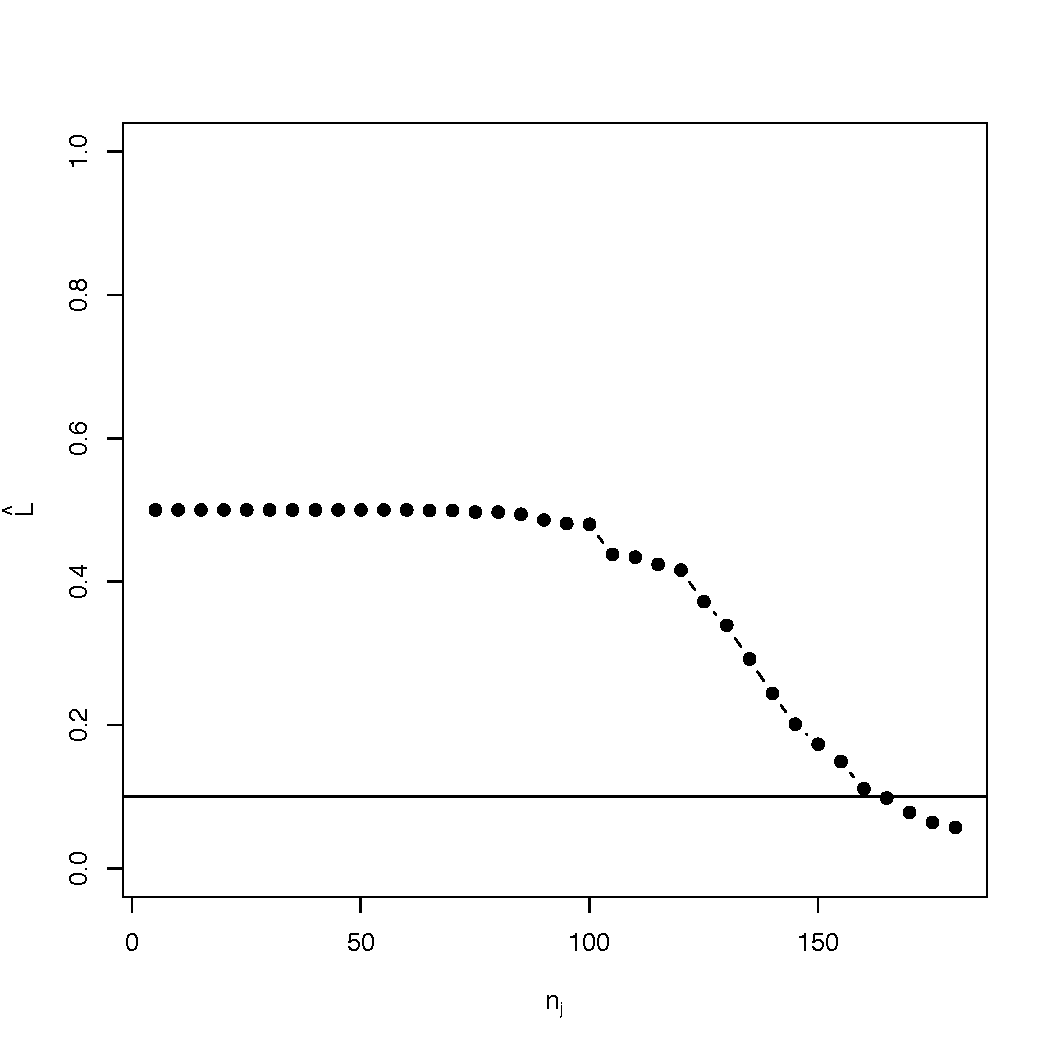
\includegraphics[width=.5\linewidth]{Lhatplot}
\caption{C.~elegans graph classification simulation results. $\hL^{1000}_{F}(g_n)$ is plotted as a function of class-conditional training sample size $n_j$, suggesting that for $\varepsilon=0.1$ we can determine that $\MeB$ holds with $99\%$ confidence with just a few hundred training samples generated from $F_{BM}$. Each dot depicts an estimate for $L_{F}(g_n)$; standard errors are $(L_{F}(g_n)(1-L_{F}(g_n))/1000)^{1/2}$. E.g., $n_j = 180$ ; $k_n = 53$ ; $\hL^{1000}_{F}(g_n) = 0.057$; standard error less than 0.01. We reject $H_0: L_{F}(g^*) \geq 0.10$ at $\alpha=0.01$. $L_{F}(g^*) \approx 0$ for this simulation.
}
\label{fig1}
\end{figure}


%% For Tables, put caption above table
%%
%% Table caption should start with a capital letter, continue with lower case
%% and not have a period at the end
%% Using @{\vrule height ?? depth ?? width0pt} in the tabular preamble will
%% keep that much space between every line in the table.

%% \begin{table}
%% \caption{Repeat length of longer allele by age of onset class}
%% \begin{tabular}{@{\vrule height 10.5pt depth4pt  width0pt}lrcccc}
%% table text
%% \end{tabular}
%% \end{table}

%% For two column figures and tables, use the following:

%% \begin{figure*}
%% \caption{Almost Sharp Front}\label{afoto}
%% \end{figure*}

%% \begin{table*}
%% \caption{Repeat length of longer allele by age of onset class}
%% \begin{tabular}{ccc}
%% table text
%% \end{tabular}
%% \end{table*}

\end{document}

